%% bare_conf.tex
%% V1.3
%% 2007/01/11
%% by Michael Shell
%% See:
%% http://www.michaelshell.org/
%% for current contact information.
%%
%% This is a skeleton file demonstrating the use of IEEEtran.cls
%% (requires IEEEtran.cls version 1.7 or later) with an IEEE conference paper.
%%
%% Support sites:
%% http://www.michaelshell.org/tex/ieeetran/
%% http://www.ctan.org/tex-archive/macros/latex/contrib/IEEEtran/
%% and
%% http://www.ieee.org/


%
\documentclass[10pt, conference, compsocconf]{IEEEtran}
% Add the compsocconf option for Computer Society conferences.
%
% If IEEEtran.cls has not been installed into the LaTeX system files,
% manually specify the path to it like:
% \documentclass[conference]{../sty/IEEEtran}





% Some very useful LaTeX packages include:
% (uncomment the ones you want to load)

\usepackage{graphicx}
% *** MISC UTILITY PACKAGES ***
%
%\usepackage{ifpdf}
\usepackage{booktabs}
\usepackage{multirow}
% Heiko Oberdiek's ifpdf.sty is very useful if you need conditional
% compilation based on whether the output is pdf or dvi.
% usage:
% \ifpdf
%   % pdf code
% \else
%   % dvi code
% \fi
% The latest version of ifpdf.sty can be obtained from:
% http://www.ctan.org/tex-archive/macros/latex/contrib/oberdiek/
% Also, note that IEEEtran.cls V1.7 and later provides a builtin
% \ifCLASSINFOpdf conditional that works the same way.
% When switching from latex to pdflatex and vice-versa, the compiler may
% have to be run twice to clear warning/error messages.

% *** CITATION PACKAGES ***
%
%\usepackage{cite}
% cite.sty was written by Donald Arseneau
% V1.6 and later of IEEEtran pre-defines the format of the cite.sty package
% \cite{} output to follow that of IEEE. Loading the cite package will
% result in citation numbers being automatically sorted and properly
% "compressed/ranged". e.g., [1], [9], [2], [7], [5], [6] without using
% cite.sty will become [1], [2], [5]--[7], [9] using cite.sty. cite.sty's
% \cite will automatically add leading space, if needed. Use cite.sty's
% noadjust option (cite.sty V3.8 and later) if you want to turn this off.
% cite.sty is already installed on most LaTeX systems. Be sure and use
% version 4.0 (2003-05-27) and later if using hyperref.sty. cite.sty does
% not currently provide for hyperlinked citations.
% The latest version can be obtained at:
% http://www.ctan.org/tex-archive/macros/latex/contrib/cite/
% The documentation is contained in the cite.sty file itself.
\usepackage[brazil]{babel}
\usepackage[utf8]{inputenc}

% *** GRAPHICS RELATED PACKAGES ***
%
\ifCLASSINFOpdf
  % \usepackage[pdftex]{graphicx}
  % declare the path(s) where your graphic files are
  % \graphicspath{{../pdf/}{../jpeg/}}
  % and their extensions so you won't have to specify these with
  % every instance of \includegraphics
  % \DeclareGraphicsExtensions{.pdf,.jpeg,.png}
\else
  % or other class option (dvipsone, dvipdf, if not using dvips). graphicx
  % will default to the driver specified in the system graphics.cfg if no
  % driver is specified.
  % \usepackage[dvips]{graphicx}
  % declare the path(s) where your graphic files are
  % \graphicspath{{../eps/}}
  % and their extensions so you won't have to specify these with
  % every instance of \includegraphics
  % \DeclareGraphicsExtensions{.eps}
\fi
% graphicx was written by David Carlisle and Sebastian Rahtz. It is
% required if you want graphics, photos, etc. graphicx.sty is already
% installed on most LaTeX systems. The latest version and documentation can
% be obtained at: 
% http://www.ctan.org/tex-archive/macros/latex/required/graphics/
% Another good source of documentation is "Using Imported Graphics in
% LaTeX2e" by Keith Reckdahl which can be found as epslatex.ps or
% epslatex.pdf at: http://www.ctan.org/tex-archive/info/
%
% latex, and pdflatex in dvi mode, support graphics in encapsulated
% postscript (.eps) format. pdflatex in pdf mode supports graphics
% in .pdf, .jpeg, .png and .mps (metapost) formats. Users should ensure
% that all non-photo figures use a vector format (.eps, .pdf, .mps) and
% not a bitmapped formats (.jpeg, .png). IEEE frowns on bitmapped formats
% which can result in "jaggedy"/blurry rendering of lines and letters as
% well as large increases in file sizes.
%
% You can find documentation about the pdfTeX application at:
% http://www.tug.org/applications/pdftex





% *** MATH PACKAGES ***
%
%\usepackage[cmex10]{amsmath}
% A popular package from the American Mathematical Society that provides
% many useful and powerful commands for dealing with mathematics. If using
% it, be sure to load this package with the cmex10 option to ensure that
% only type 1 fonts will utilized at all point sizes. Without this option,
% it is possible that some math symbols, particularly those within
% footnotes, will be rendered in bitmap form which will result in a
% document that can not be IEEE Xplore compliant!
%
% Also, note that the amsmath package sets \interdisplaylinepenalty to 10000
% thus preventing page breaks from occurring within multiline equations. Use:
%\interdisplaylinepenalty=2500
% after loading amsmath to restore such page breaks as IEEEtran.cls normally
% does. amsmath.sty is already installed on most LaTeX systems. The latest
% version and documentation can be obtained at:
% http://www.ctan.org/tex-archive/macros/latex/required/amslatex/math/





% *** SPECIALIZED LIST PACKAGES ***
%
%\usepackage{algorithmic}
% algorithmic.sty was written by Peter Williams and Rogerio Brito.
% This package provides an algorithmic environment fo describing algorithms.
% You can use the algorithmic environment in-text or within a figure
% environment to provide for a floating algorithm. Do NOT use the algorithm
% floating environment provided by algorithm.sty (by the same authors) or
% algorithm2e.sty (by Christophe Fiorio) as IEEE does not use dedicated
% algorithm float types and packages that provide these will not provide
% correct IEEE style captions. The latest version and documentation of
% algorithmic.sty can be obtained at:
% http://www.ctan.org/tex-archive/macros/latex/contrib/algorithms/
% There is also a support site at:
% http://algorithms.berlios.de/index.html
% Also of interest may be the (relatively newer and more customizable)
% algorithmicx.sty package by Szasz Janos:
% http://www.ctan.org/tex-archive/macros/latex/contrib/algorithmicx/




% *** ALIGNMENT PACKAGES ***
%
%\usepackage{array}
% Frank Mittelbach's and David Carlisle's array.sty patches and improves
% the standard LaTeX2e array and tabular environments to provide better
% appearance and additional user controls. As the default LaTeX2e table
% generation code is lacking to the point of almost being broken with
% respect to the quality of the end results, all users are strongly
% advised to use an enhanced (at the very least that provided by array.sty)
% set of table tools. array.sty is already installed on most systems. The
% latest version and documentation can be obtained at:
% http://www.ctan.org/tex-archive/macros/latex/required/tools/


%\usepackage{mdwmath}
%\usepackage{mdwtab}
% Also highly recommended is Mark Wooding's extremely powerful MDW tools,
% especially mdwmath.sty and mdwtab.sty which are used to format equations
% and tables, respectively. The MDWtools set is already installed on most
% LaTeX systems. The lastest version and documentation is available at:
% http://www.ctan.org/tex-archive/macros/latex/contrib/mdwtools/


% IEEEtran contains the IEEEeqnarray family of commands that can be used to
% generate multiline equations as well as matrices, tables, etc., of high
% quality.


%\usepackage{eqparbox}
% Also of notable interest is Scott Pakin's eqparbox package for creating
% (automatically sized) equal width boxes - aka "natural width parboxes".
% Available at:
% http://www.ctan.org/tex-archive/macros/latex/contrib/eqparbox/





% *** SUBFIGURE PACKAGES ***
%\usepackage[tight,footnotesize]{subfigure}
% subfigure.sty was written by Steven Douglas Cochran. This package makes it
% easy to put subfigures in your figures. e.g., "Figure 1a and 1b". For IEEE
% work, it is a good idea to load it with the tight package option to reduce
% the amount of white space around the subfigures. subfigure.sty is already
% installed on most LaTeX systems. The latest version and documentation can
% be obtained at:
% http://www.ctan.org/tex-archive/obsolete/macros/latex/contrib/subfigure/
% subfigure.sty has been superceeded by subfig.sty.



%\usepackage[caption=false]{caption}
%\usepackage[font=footnotesize]{subfig}
% subfig.sty, also written by Steven Douglas Cochran, is the modern
% replacement for subfigure.sty. However, subfig.sty requires and
% automatically loads Axel Sommerfeldt's caption.sty which will override
% IEEEtran.cls handling of captions and this will result in nonIEEE style
% figure/table captions. To prevent this problem, be sure and preload
% caption.sty with its "caption=false" package option. This is will preserve
% IEEEtran.cls handing of captions. Version 1.3 (2005/06/28) and later 
% (recommended due to many improvements over 1.2) of subfig.sty supports
% the caption=false option directly:
%\usepackage[caption=false,font=footnotesize]{subfig}
%
% The latest version and documentation can be obtained at:
% http://www.ctan.org/tex-archive/macros/latex/contrib/subfig/
% The latest version and documentation of caption.sty can be obtained at:
% http://www.ctan.org/tex-archive/macros/latex/contrib/caption/




% *** FLOAT PACKAGES ***
%
%\usepackage{fixltx2e}
% fixltx2e, the successor to the earlier fix2col.sty, was written by
% Frank Mittelbach and David Carlisle. This package corrects a few problems
% in the LaTeX2e kernel, the most notable of which is that in current
% LaTeX2e releases, the ordering of single and double column floats is not
% guaranteed to be preserved. Thus, an unpatched LaTeX2e can allow a
% single column figure to be placed prior to an earlier double column
% figure. The latest version and documentation can be found at:
% http://www.ctan.org/tex-archive/macros/latex/base/



%\usepackage{stfloats}
% stfloats.sty was written by Sigitas Tolusis. This package gives LaTeX2e
% the ability to do double column floats at the bottom of the page as well
% as the top. (e.g., "\begin{figure*}[!b]" is not normally possible in
% LaTeX2e). It also provides a command:
%\fnbelowfloat
% to enable the placement of footnotes below bottom floats (the standard
% LaTeX2e kernel puts them above bottom floats). This is an invasive package
% which rewrites many portions of the LaTeX2e float routines. It may not work
% with other packages that modify the LaTeX2e float routines. The latest
% version and documentation can be obtained at:
% http://www.ctan.org/tex-archive/macros/latex/contrib/sttools/
% Documentation is contained in the stfloats.sty comments as well as in the
% presfull.pdf file. Do not use the stfloats baselinefloat ability as IEEE
% does not allow \baselineskip to stretch. Authors submitting work to the
% IEEE should note that IEEE rarely uses double column equations and
% that authors should try to avoid such use. Do not be tempted to use the
% cuted.sty or midfloat.sty packages (also by Sigitas Tolusis) as IEEE does
% not format its papers in such ways.





% *** PDF, URL AND HYPERLINK PACKAGES ***
%
\usepackage{url}
% url.sty was written by Donald Arseneau. It provides better support for
% handling and breaking URLs. url.sty is already installed on most LaTeX
% systems. The latest version can be obtained at:
% http://www.ctan.org/tex-archive/macros/latex/contrib/misc/
% Read the url.sty source comments for usage information. Basically,
% \url{my_url_here}.

\providecommand{\natexlab}[1]{#1}
\providecommand{\url}[1]{\texttt{#1}}
\expandafter\ifx\csname urlstyle\endcsname\relax
  \providecommand{\doi}[1]{doi: #1}\else
  \providecommand{\doi}{doi: \begingroup \urlstyle{rm}\Url}\fi






% *** Do not adjust lengths that control margins, column widths, etc. ***
% *** Do not use packages that alter fonts (such as pslatex).         ***
% There should be no need to do such things with IEEEtran.cls V1.6 and later.
% (Unless specifically asked to do so by the journal or conference you plan
% to submit to, of course. )


% correct bad hyphenation here
\hyphenation{op-tical net-works semi-conduc-tor}


\begin{document}
%
% paper title
% can use linebreaks \\ within to get better formatting as desired
\title{Predizendo Vendas em Telemarketing Bancário}


% author names and affiliations
% use a multiple column layout for up to two different
% affiliations

\author{\IEEEauthorblockN{Charles D. Moraes, Henrique T. Eihara, João Victor do C. Binatto, Rafael  F. Zanetti}
\IEEEauthorblockA{Departamento de Computação (DComp)\\
Universidade Federal de São Carlos (UFSCar) \\
18052-780, Sorocaba, São Paulo, Brasil \\
raverblazer@gmail.com, rick.eihara@gmail.com, joaovictorbinatto@hotmail.com, rfzanetti@gmail.com}
}

% conference papers do not typically use \thanks and this command
% is locked out in conference mode. If really needed, such as for
% the acknowledgment of grants, issue a \IEEEoverridecommandlockouts
% after \documentclass

% for over three affiliations, or if they all won't fit within the width
% of the page, use this alternative format:
% 
%\author{\IEEEauthorblockN{Michael Shell\IEEEauthorrefmark{1},
%Homer Simpson\IEEEauthorrefmark{2},
%James Kirk\IEEEauthorrefmark{3}, 
%Montgomery Scott\IEEEauthorrefmark{3} and
%Eldon Tyrell\IEEEauthorrefmark{4}}
%\IEEEauthorblockA{\IEEEauthorrefmark{1}School of Electrical and Computer Engineering\\
%Georgia Institute of Technology,
%Atlanta, Georgia 30332--0250\\ Email: see http://www.michaelshell.org/contact.html}
%\IEEEauthorblockA{\IEEEauthorrefmark{2}Twentieth Century Fox, Springfield, USA\\
%Email: homer@thesimpsons.com}
%\IEEEauthorblockA{\IEEEauthorrefmark{3}Starfleet Academy, San Francisco, California 96678-2391\\
%Telephone: (800) 555--1212, Fax: (888) 555--1212}
%\IEEEauthorblockA{\IEEEauthorrefmark{4}Tyrell Inc., 123 Replicant Street, Los Angeles, California 90210--4321}}




% use for special paper notices
%\IEEEspecialpapernotice{(Invited Paper)}




% make the title area
\maketitle


\begin{abstract}
As empresas cada vez mais se utilizam de diferentes formas para agregar novos clientes à seus produtos. Uma das formas de atingir seus clientes é por campanhas de telemarketing, em que a prospecção de vendas se classficam como: \emph{inbound} (quando o cliente tem a pró-atividade em comprar o produto), \emph{outbound} (quando um intermediário oferece tal produto diretamente pro cliente). É extremamente importante identificar os possíveis clientes para que seja possível maximizar a prospecção de vendas do produto, dessa forma, utilizando de Sistemas de Suporte à Decisão em conjunto com algoritmos de Aprendizado de Máquina, é possível identificar com eficiência quem são os melhores clientes para se oferecer tal produto. Diante deste cenário, esse trabalho apresenta uma análise de técnicas de aprendizado de máquina aplicados na classificação dos melhores clientes. Utilizando uma base de dados real criada por um banco português, em sua campanha de marketing, foi possível realizar experimentos utilizando os algoritmos k-vizinhos mais próximos, regressão logística, redes neurais e máquina de vetores de suporte; resultados obtidos nos nossos experimentos indicaram que o uso de regressão logística é apropriado para construção de um modelo promissor na identificação dos usuários que tem uma maior chance de aderir à venda proporcionada por uma campanha de telemarketing.

\end{abstract}

\begin{IEEEkeywords}
telemarketing bancário; vendas; classificação.
\end{IEEEkeywords}
% For peer review papers, you can put extra information on the cover
% page as needed:
% \ifCLASSOPTIONpeerreview
% \begin{center} \bfseries EDICS Category: 3-BBND \end{center}
% \fi
%
% For peerreview papers, this IEEEtran command inserts a page break and
% creates the second title. It will be ignored for other modes.
\IEEEpeerreviewmaketitle


\section{Introdução}
As empresas cada vez mais se utilizam de diferentes formas para agregar novos clientes à seus produtos. Uma dessas formas é por meio de campanhas de telemarketing, forma que nasceu e cresceu na década 19 com a popularização do telefone. Com as empresas, cada vez mais com uma demanda maior para vender seus produtos, diversos empregos como Operador de Telemarketing foram criados, além de ser uma forma barata de campanha, é uma das formas em que mais clientes são atingidos.

Há duas classificações das prospecções de vendas de telemarketing, sendo elas,  \emph{inbound}, quando é o cliente que realiza a ligação para a empresa com interesse de comprar o produto, e \emph{outbound}, quando o Operador de Telemarketing realiza a oferta de um produto para um cliente. Para ter êxito nas vendas do produto, é imprescindível conhecer o público alvo do produto e também o perfil do cliente que irá ser oferecido, dessa forma, escolher o melhor conjunto de clientes que poderão comprar o produto pode ser considerado parte do conjunto de problemas NP-Difícil \cite{np_dificil}.

Nesta situação, umas das soluções é a utilização de Sistemas de Suporte à Decisão, em que, são sistemas que utilizam um modelo genérico de tomada de decisão e tem como base sua análise em um grande conjunto de variáveis, dessa forma, através da análise dos dados é possível determinar um posicionamento e/ou escolha \cite{administracao_sistemas}.

Muitos algoritmos de classificação são utilizados em Sistemas de Suporte à Decisão, sendo eles o k-vizinhos próximos, regressão logística, árvores de decisão, redes neurais, e ainda os mais recentes, Deep Learning (redes neurais) e máquinas de vetores de suporte que é o estado da arte na área de Aprendizado de Máquina. \cite{rule_extraction}

Neste artigo iremos avaliar o desempenho dos métodos de aprendizado de máquinas: k-vizinhos próximos, regressão logística, redes neurais e máquinas de vetores de suporte. Esses métodos poderão ser utilizados para aumentar a prospecção de venda de produtos, a partir da classificação do perfil dos clientes de uma campanha de telemarketing. O objetivo principal é realizar uma análise dos métodos de classificação em conjunto com os possíveis parâmetros promissores deste cenário.

Este artigo está estruturado da seguinte forma, na Seção II está apresentado a modelagem da base de dados, além de sua origem e características. Na Seção III é apresentado os métodos de aprendizado de máquina, seus parâmetros de configuração e suas características. Na Seção IV encontra-se os resultados obtidos a partir da execução desses métodos de classificação, e por último, na Seção V, são apresentadas as principais conclusões e análises deste trabalho.

 \section{Dados Utilizados}
	Nesta seção é apresentada a base de dados utilizada neste trabalho, juntamente com o processo de pré-processamento realizado para possibilitar o uso dos algoritmos desejados.
    
    A base de dados original foi apresentada por \cite{bank_dataset} e contém dados de uma campanha de marketing de um banco de Portugal com 41.188 amostras com 21 atributos referentes às seguintes categorias:
\begin{itemize}
  \item Dados do cliente contatado:
      \begin{itemize}
          \item idade, profissão, estado civil, escolaridade, situação de inadimplência de crédito, existência de empréstimos pessoais e relacionados à moradia.
      \end{itemize}
  \item Dados do último contato relacionado à campanha: 
      \begin{itemize} 
          \item tipo do contato (telefone fixo ou móvel), mês, dia da semana e duração, em minutos. 
      \end{itemize}
  \item Dados de contexto social e econômico:
      \begin{itemize}
          \item  índice de desemprego (trimestral), índice de preços no consumidor (mensal), índice de confiança do consumidor (mensal), taxa interbancária oferecida em euro (diário) e número de empregados (trimestral).
      \end{itemize}
  \item  Outros:
      \begin{itemize} 
          \item numero de contatos com o cliente na campanha, número de dias do último contato relacionado a alguma campanha e resultado desta, e número de contatos com o cliente antes da campanha em questão. 
      \end{itemize}
     \item  Resultado:
      \begin{itemize} 
          \item O sucesso ou não da campanha.
      \end{itemize}
\end{itemize} 


Após uma análise inicial dos dados, optou-se por remover o atributo relacionado à inadimplência, pois apenas três amostras no conjunto tinham valor positivo, e a maioria das amostras não tinha informação sobre seu valor.

Após essa remoção, a base ainda apresentava o problema de um número considerável de amostras com pelo menos um atributo faltando (aproximadamente 7\% da base), o que prejudicava a aplicação dos algoritmos desejados. Pela disponibilidade de um número satisfatório de amostras, optou-se pela sua remoção, resultando em 38.247 amostras restantes.

O atributo relacionado ao número de dias desde o último contato foi notado como possível problema para os algoritmos, pois, nos dados, a representação de uma situação em que esse contato não existiu foi definida pelos seus criadores com o valor 999. Para os algoritmos, seria uma diferença extrema entre os outros valores, visto que o valor máximo apresentado na base é 33. Para lidar com isso, decidiu-se utilizar o valor 50 nessas situações, mantendo assim uma diferenciação razoável para casos em que esse contato existiu anteriormente e casos nos quais ele não existiu.

Outro problema encontrado foi a presença de atributos nominais, como por exemplo a profissão do cliente, o que complicava a utilização dos dados. Para tratá-lo, duas abordagens distintas foram tomadas:

\begin{itemize}
\item Para o atributo \emph{escolaridade}, cujos valores nominais representam uma escala bem definida, os valores (\emph{analfabeto, básico (4 anos), básico (6 anos), básico (9 anos), médio, superior, pós-graduação}) foram mapeados numa escala de 0 a 6.
\item Cada um dos outros atributos nominais, cujo domínio não possibilita a abordagem acima, foi transformado em $n$ atributos binários (sendo $n$ o número de diferentes valores presentes). Por exemplo, o atributo \emph{estado civil}, que apresentava os valores \emph{solteiro, casado} e \emph{divorciado}, foi mapeado em \emph{bool-solteiro, bool-casado} e \emph{bool-divorciado}. Exemplificando, valores de, respectivamente, \emph{0, 1} e \emph{0} nesses atributos são usados para representar o valor \emph{casado} no atributo original. 
\end{itemize}

Após o procedimento descito acima, totalizou-se 34 atributos na base. Analisando a distribuição de classes no conjunto de dados, restaram 33.988 amostras negativas e 4,258 amostras positivas. Em experimentos iniciais, verificou-se que, apesar de os algoritmos aplicados terem obtido bons níveis de acurácia, essa disparidade entre classes fazia com que a revocação da classe minoritária fosse baixa, ou seja, eles tendiam a classificar novas amostras na classe majoritária. 

Para tratar esse problema, foram realizados testes com diferentes proporções de amostras positivas e negativas (com \emph{undersampling}), avaliando sempre o MCC (\emph{Matthews Correlation Coefficient}). 

\begin{table}[ht]
	\centering
  \begin{tabular}{ | c | c | c |}
    \hline
     & Amostras positivas & Amostras negativas \\ \hline
    Antes & 4258 & 33988 \\ \hline
    Depois & 4258 & 4258 \\
    \hline
  \end{tabular}
  \caption{Distribuição de amostras antes e depois do balanceamento}
  \label{tab:tabela_amostra}
\end{table}

Os melhores resultados foram obtidos com o mesmo número de amostras nas duas classes, portanto decidiu-se pela remoção de amostras negativas aleatóriamente para ter uma base perfeitamente balanceada. A Tabela \ref{tab:tabela_amostra} apresenta a distribuição de classes antes e depois do processo de balanceamento.
   
\section{Metodologia Experimental}

Foram definidos quatro algoritmos a serem utilizados para os experimentos de Aprendizado de Máquina: k-vizinhos mais próximos (\emph{k-NN}) \cite{knn}, regressão logística \cite{logistic}, redes neurais artificiais \cite{neural_networks} e máquina de vetores de suporte (\emph{SVM}) \cite{svm}. As próximas subseções reportam as metodologias experimentais gerais e específicas para cada algoritmo.

\subsection{Implementação}
Todos os algoritmos foram implementados utilizando \emph{GNU Octave}.

\subsection{Avaliação}
Para avaliar a capacidade de generalização dos modelos construídos e evitar o super-ajustamento (\emph{overfitting}), foi selecionada a técnica de validação cruzada com $k$ partições, utilizando $k = 5$. 

\subsection{Métricas}
As seguintes métricas foram escolhidas para avaliar o desempenho dos modelos construídos:

\begin{itemize}
\item Acurácia - porcentagem de amostras classificadas corretamente
\item F-Medida - media harmônica entre precisão e revocação
\item MCC (\emph{Matthews Correlation Coefficient}) - medida de qualidade de classificações binárias
\end{itemize}

\subsection{Normalização e Redução de Dimensionalidade}
Uma técnica comumente utilizada para algoritmos de Aprendizado de Máquina é a normalização dos dados, para que o conjunto de valores de cada atributo tenha média 0 e desvio padrão 1, de modo que todos os atributos estejam na mesma escala. 

Outra prática comum é a aplicação do PCA (Análise de Componentes Principais) para reduzir a dimensionalidade dos dados, com diferentes motivações (como por exemplo, a aceleração do treinamento). 

Como os algoritmos a serem implementados tem propriedades bem distintas entre si, a aplicação das técnicas citadas acima foi avaliada separadamente para cada um. Essas avaliações, juntamente com metodologias especificas para cada algoritmo, são apresentadas nas subseções abaixo.

\subsection{K-vizinhos mais próximos}
 
Nos experimentos com o algoritmo k-vizinhos mais próximos, foram identificados problemas de acurácia devido à dimensionalidade dos dados. Devido a isso, o algoritmo apresentou problemas na classificação dos dados de teste, apresentando vários casos onde a distância de diversas amostras ficou idêntica, assim comprometendo o agrupamento dos k-vizinhos. 

O cálculo da distância, inicialmente Euclidiana, foi modificado para \emph{Manhattan} e posteriormente \emph{Minkowski}, entretanto tais mudanças não refletiram numa melhora real na acurácia. Portanto, optou-se por continuar utilizando a distância Euclidiana.

Para tentar contornar os resultados insatisfatórios, foi utilizada a técnica do PCA (Análise das Componentes Principais) para reduzir a dimensionalidade da base, mantendo 95\% de variância dos dados. Verificou-se uma melhora, porém não muito expressiva.

Finalmente, foram realizados testes com $K = 1, 3, 5, 7, 9$, e foi escolhido $K=7$ por apresentar os melhores resultados.

\subsection{Regressão Logística}

Em experimentos preliminares, os resultados obtidos com a aplicação da Regressão Logística foram surpreendentemente eficazes. Porém, ao realizar testes com normalização dos dados, os resultados chegaram a melhorar ainda mais. Por isso, a normalização dos dados foi aplicada nos experimentos.

Com resultados satisfatórios e execução rápida, a redução de dimensionalidade não se mostrou necessária e não foi aplicada.

Para tentar aprimorar ainda mais os resultados, foi realizada uma busca pelo valor $\lambda$ ótimo da regressão, sendo feita uma busca utilizando os valores 0, 0.01, 0, 05, 0.10, 0.25, 0.5, 0.75 e 1. O valor 0.01 apresentou os melhores resultados e foi selecionado para os experimentos.
\subsection{Redes Neurais Artificiais}

Em experimentos iniciais, os resultados indicaram uma classificação ruim e inconsistente, e uma análise mais profunda indicou que a otmização da função custo apresentava uma considerável demora para convergir. Um modo de corrigir esse problema é a normalização do conjunto de dados \cite{backprop}. Testes com a aplicação dessa técnica apontaram resultados melhores e mais consistentes, portanto decidiu-se pela aplicação de normalização.

Foram realizados testes com redução de dimensionalidade, porém a diferença no tempo dos experimentos não foi grande o suficiente pra justificar a piora nos resultados devido à perda de variância dos dados.

Um dos parâmetros do algoritmo é a quantidade de iterações para otimização da função custo. A Figura \ref{fig:grafico_nn} corresponde a uma curva que apresenta a relação entre valor da função custo e número de iterações:

\begin{figure}[ht]
  \centering
    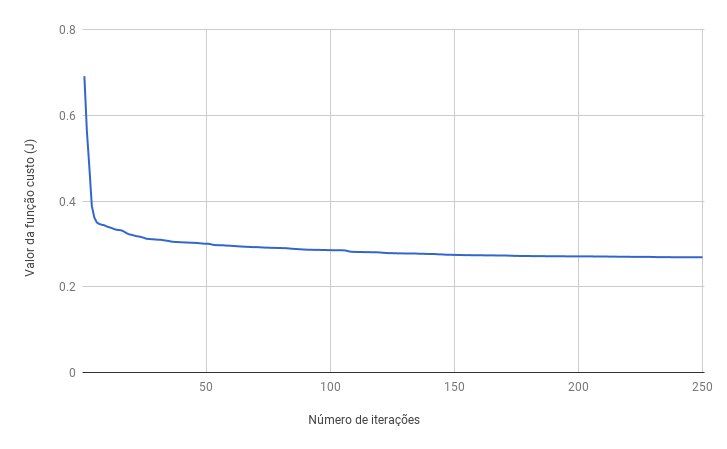
\includegraphics[width=0.5\textwidth]{chart.png}
    \caption{Curva de relação entre número de iterações e valor da função custo}
    \label{fig:grafico_nn}
\end{figure}


De acordo com a curva, foi escolhido o valor de 75 iterações, por se tratar de um ponto onde a execução não é excessiva, porém com um nível satisfatório de otimização para a função custo.

Por fim, dois parâmetros inteferem diretamente no desempenho: o número de nós na camada intermediária, e o $\lambda$ utilizado na regularização dos pesos. Para otimizá-los, foi realizada uma busca em \emph{grid}, onde os seguintes valores foram testados, utilizando o MCC como referência para comparação:

\begin{itemize}
\item Número de nós: De $3$ a $25$.
\item $\lambda$: $0, 0.01, 0,05, 0.10, 0.25, 0.5, 0.75, 1$.
\end{itemize}

Após a busca, foram os selecionados 6 nós na camada intermediária e $\lambda = 0.05$. 
\subsection{Máquinas de vetores de suporte}

Para implementar a técnica de máquinas de vetores de suporte utilizamos a conhecida biblioteca LIBSVM \cite{libsvm} e também uma breve leitura inicial de um guia \cite{libsvm_guide}, disponibilizado pelos principais responsáveis pela biblioteca.

Seguindo as recomendações providas pelo guia, iniciamos alguns testes com a função \emph{kernel} Gaussiana (\emph{Radial Basis Function}), dada por:

\begin{equation}
	K(x, y) = e^{-\gamma ||x - y||^2}
\end{equation}

Portanto, temos 2 hiperparâmetros a serem escolhidos, $C$ e $\gamma$. Sendo $C$ o parâmetro de penalização, ou seja, é o \emph{trade-off} entre classificar uma amostra de treino erroneamente contra a simplificação da superfície de decisão. Um valor baixo resulta em uma fronteira de decisão suave, e quanto maior o valor, maior a tendência de classificar todas as amostras de treino corretamente, dando ao modelo plena liberdade de escolher mais amostras como vetores de suporte.

Já o parâmetro $\gamma$ define qual o alcance de influência de uma única amostra de treino, onde um valor baixo indica longo alcance e um valor alto indica curto alcance. Este parâmetro pode ser visto como o inverso do raio de influência das amostras selecionadas pelo modelo como vetores de suporte. É possível observar, de forma mais intuitiva e visual o comportamento destes parâmetros na Figura \ref{fig:grafico_rbf_demo}.

\begin{figure}[ht]
  \centering
    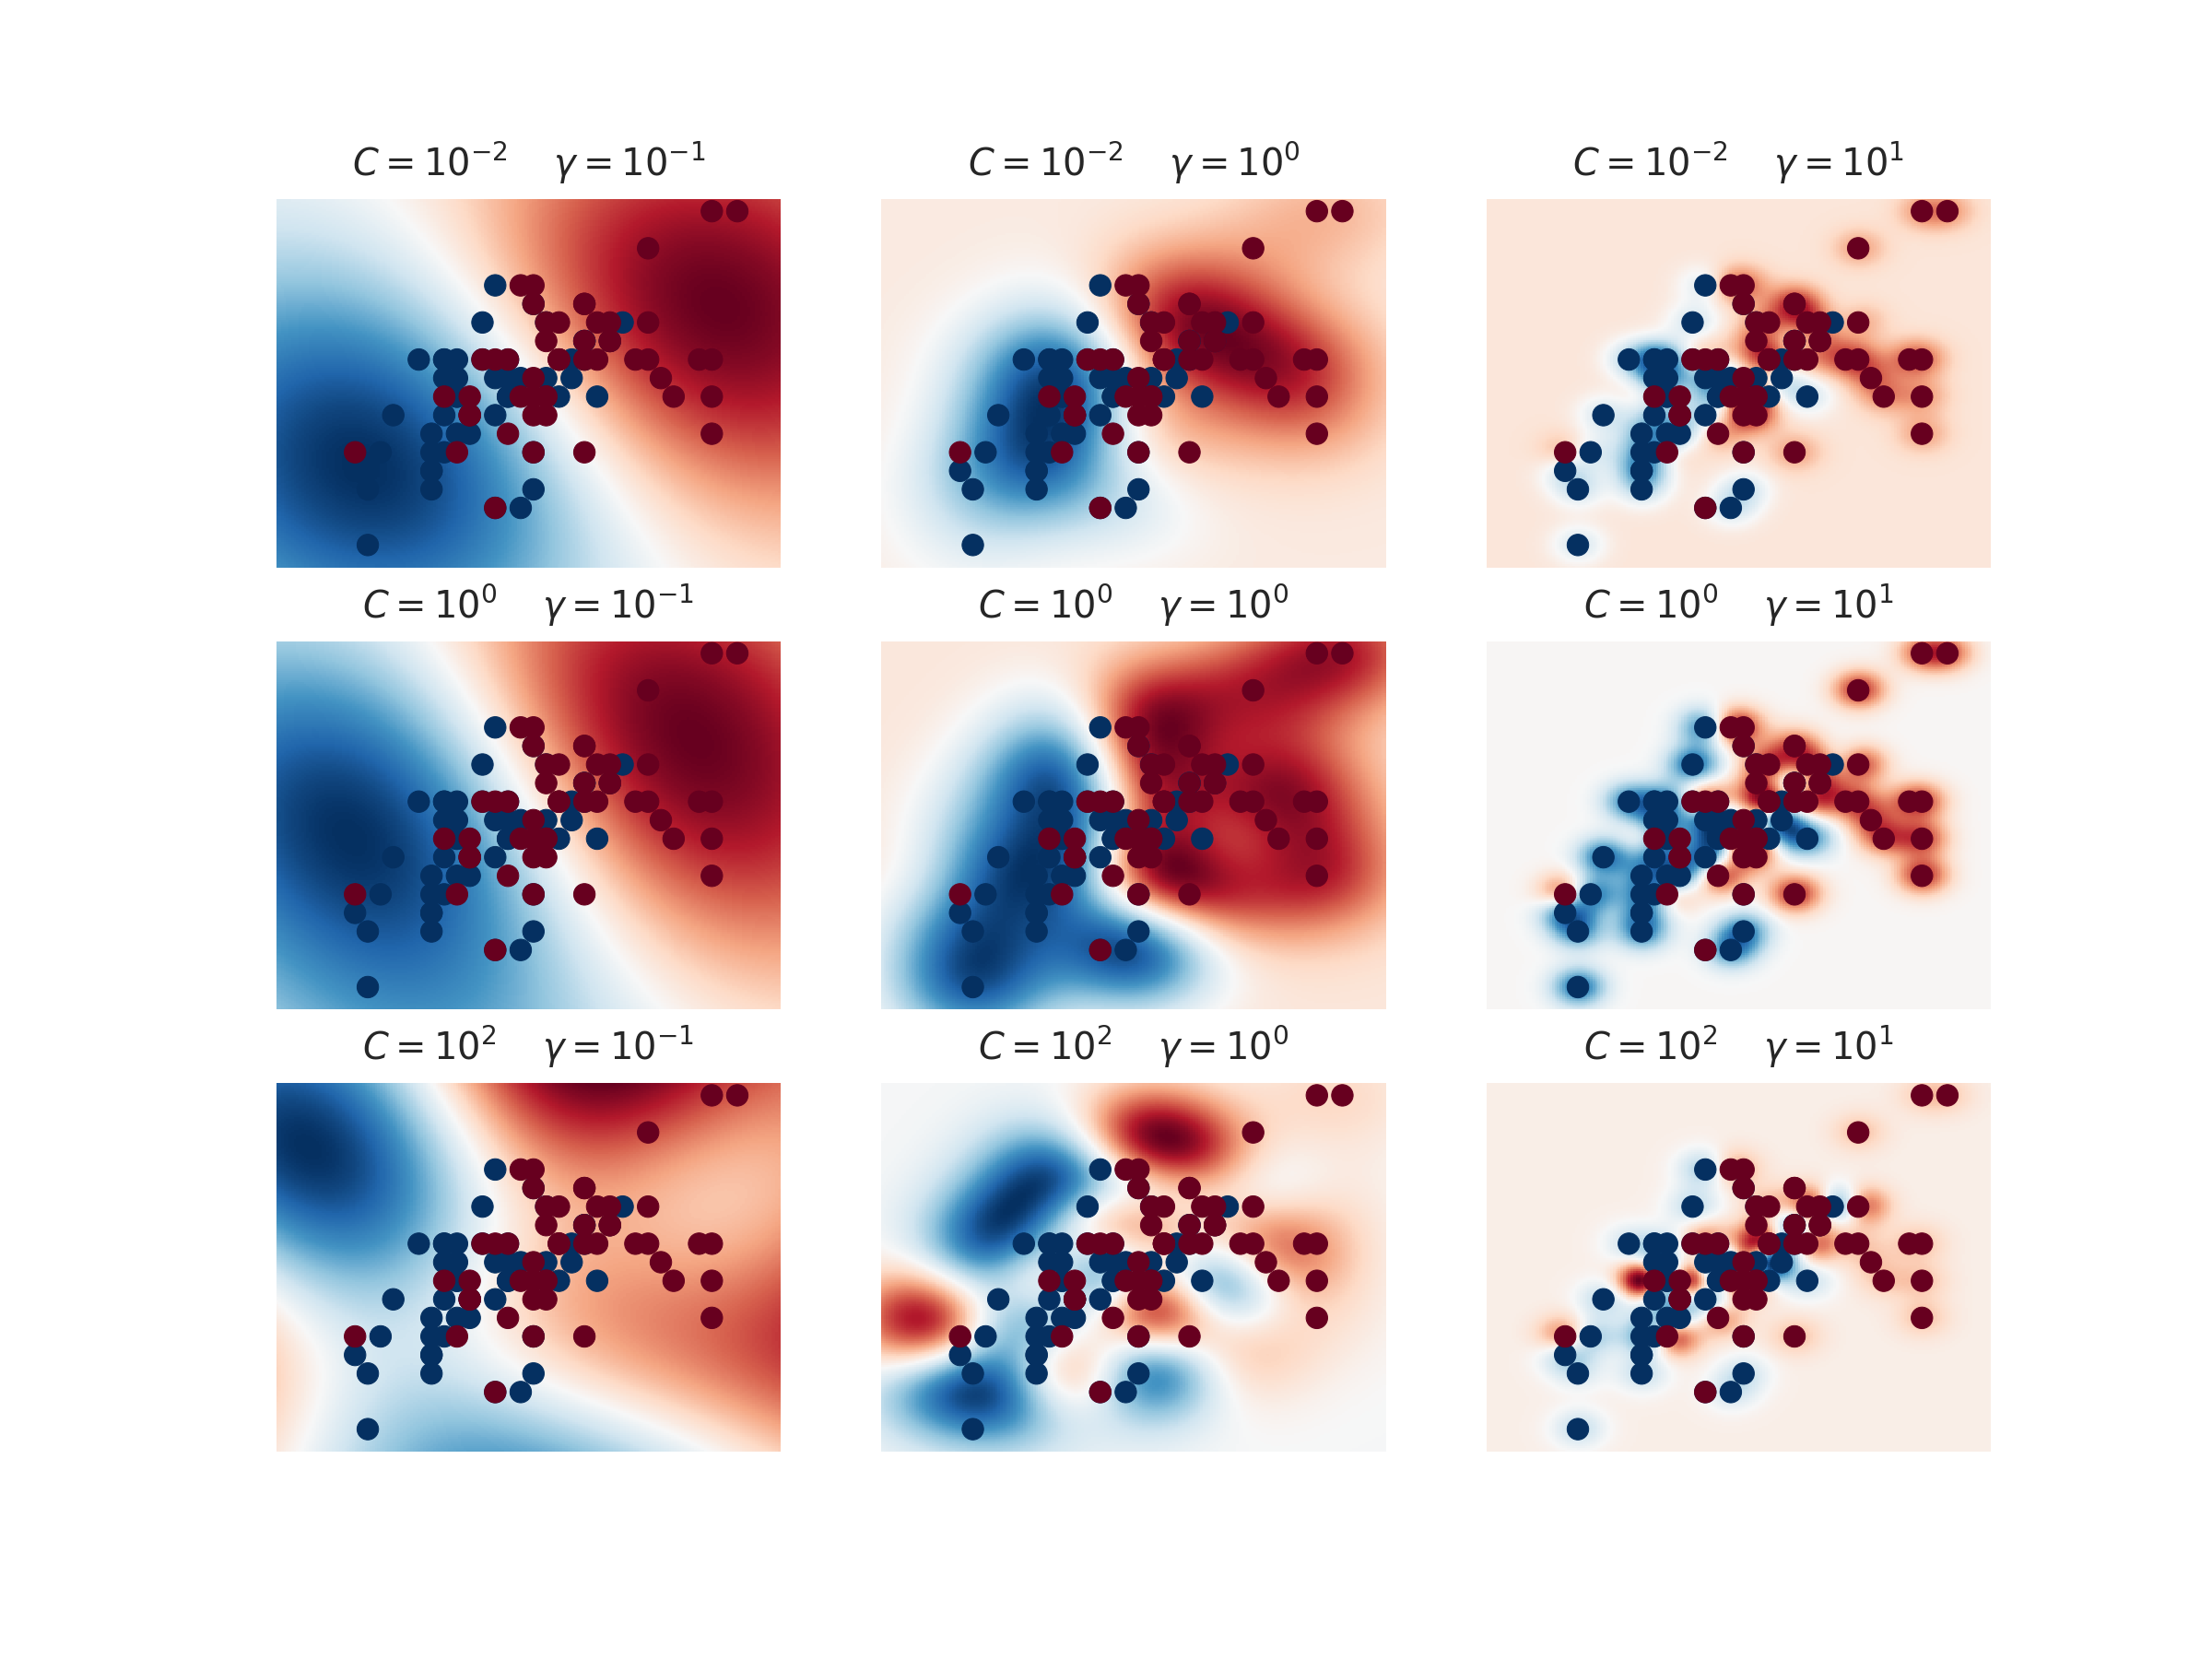
\includegraphics[width=0.5\textwidth]{rbf_hyperparams_demo.png}
    \caption{Demonstração do comportamento de $C$ e $\gamma$ utilizando como exemplo o \emph{Iris Dataset} \cite{uci_ml_repo}}
    \label{fig:grafico_rbf_demo}
\end{figure}

Após termos escolhido inicialmente o \emph{kernel} RBF para os primeiros testes, uma leitura mais a fundo mostrou também os seguintes pontos importantes que nos levaram a escolha definitiva desta função \emph{kernel}.

O \emph{kernel} RBF mapeia as amostras de forma não linear para um espaço dimensional maior, portanto, pode lidar com casos onde a relação entre os atributos e a classe não são lineares. Além do mais, ele possui a mesma performance de um \emph{kernel} linear com parâmetro de penalização $\tilde{C}$  \cite{rbf_linear}.

Outro fato muito importante é o número de hiperparâmetros a serem escolhidos, os quais influenciam a complexidade de seleção do modelo. O \emph{kernel} polinomial é dado por:

\begin{equation}
	K(x, y) = (\gamma x^T y + r)^d
\end{equation}

Ou seja, temos quatro hiperparâmetros para serem selecionados: $C$, $\gamma$, $r$ e $d$. Além disso, o \emph{kernel} polinomial pode sofrer com dificuldades numéricas, onde os valores do \emph{kernel} podem tender a infinito $(\gamma x^T y + r > 1)$ ou zero $(\gamma x^T y + r < 0)$ quando o grau($d$) é alto, enquanto os valores do \emph{kernel} RBF ficam entre 0 e 1 $(0 < K_{ij} < 1)$.

Para otimizarmos os hiperparâmetros $C$ e $\gamma$ realizamos busca em \emph{grid} com \emph{5-fold cross-validation}. Segundo o guia, sequências que crescem exponencialmente são um método prático para se identificar bons parâmetros \cite{libsvm_guide}. Portanto, seguindo as recomendações do mesmo, optamos por realizar duas buscas em \emph{grid}. Ambas as buscas foram realizadas duas vezes, sendo uma aplicando PCA e outra não, e ambas com normalização dos atributos.

A primeira busca possui um intervalo mais amplo entre os valores exponenciais, sendo seu \emph{step} de $2^2$ e as seguintes sequências: $C = 2^{-5}, 2^{-3}, ..., 2^{15}$ e $\gamma = 2^{-13}, 2^{-11}, ..., 2^1$. Após realizada a primeira busca agrupamos todos os resultados por cada parâmetro e tiramos a média e desvio padrão da acurácia e MCC para identificamos os intervalos de $C$ e $\gamma$ que obtiveram os melhores resultados, como podemos obserar na Tabela \ref{tab:svm_coarse_grid_table}.

\begin{table}[ht]
\centering
\begin{tabular}{@{}lcc|ccr@{}}
\toprule
\multirow{2}{*}{} & \multicolumn{2}{c|}{$C$}                   & \multicolumn{2}{c}{$\gamma$} & \multicolumn{1}{l}{\multirow{2}{*}{}} \\ \cmidrule(lr){2-5}
                  & Acc       & MCC                        & Acc       & MCC           & \multicolumn{1}{l}{}                  \\ \midrule
$2^{-5}$          & $0.65 \pm 0.14$ & $0.32 \pm 0.28$              & $0.80 \pm 0.12$ & $0.60 \pm 0.23$ & $2^{-13}$                             \\
$2^{-3}$          & $0.73 \pm 0.13$ & $0.49 \pm 0.24$              & $0.84 \pm 0.06$ & $0.68 \pm 0.12$ & $2^{-11}$                             \\
$2^{-1}$          & $0.79 \pm 0.09$ & $0.60 \pm 0.15$              & $\bf{0.85 \pm 0.04}$ & $\bf{0.70 \pm 0.08}$ & $2^{-9}$                              \\
$2^{1}$           & $\bf{0.82 \pm 0.06}$ & $\bf{0.66 \pm 0.10}$              & $\bf{0.85 \pm 0.03}$ & $\bf{0.70 \pm 0.05}$ & $2^{-7}$                              \\
$2^{3}$           & $\bf{0.83 \pm 0.06}$ & $\bf{0.66 \pm 0.11}$              & $\bf{0.84 \pm 0.03}$ & $\bf{0.68 \pm 0.05}$ & $2^{-5}$                              \\
$2^{5}$           & $\bf{0.83 \pm 0.06}$  & $\bf{0.66 \pm 0.11}$              & $0.81 \pm 0.04$ & $0.62 \pm 0.06$ & $2^{-3}$                              \\
$2^{7}$           & $0.82 \pm 0.06$ & $0.65 \pm 0.11$              & $0.72 \pm 0.09$ & $0.47 \pm 0.18$ & $2^{-1}$                              \\
$2^{9}$           & $0.82 \pm 0.06$ & $0.65 \pm 0.11$              & $0.65 \pm 0.09$ & $0.34 \pm 0.19$ & $2^{1}$                              \\
$2^{11}$          & $0.82 \pm 0.06$ & $0.64 \pm 0.11$              &       -        &        -       & \multicolumn{1}{c}{-}                 \\
$2^{13}$          & $0.81 \pm 0.06$ & $0.63 \pm 0.11$ &  -             &       -        & \multicolumn{1}{c}{-}                 \\ \bottomrule
\end{tabular}
\caption{Resultados do \emph{Coarse Grid Search} sem PCA}
\label{tab:svm_coarse_grid_table}
\end{table}

Apesar da sequência que definimos inicialmente para $C$ ir até $2^{15}$ não chegamos a concluir a busca em \emph{grid} neste último exponencial devido ao alto custo computacional, exigindo um grande número de iterações pela SVM e demorando consideravelmente em cada \emph{fold} da validação cruzada, além disso, tanto a acurácia quanto o MCC já se encontravam em queda a partir do exponencial $2^7$.

A segunda busca possui um intervalo mais curto entre os valores exponenciais, sendo seu step de $2^{0.25}$ e as sequências obtidas a partir da primeira busca foram: $C = 2^{1}, 2^{1.25}, ..., 2^{5}$ e $\gamma = 2^{-9}, 2^{-9.25}, ..., 2^{-5}$, como pudemos observar na Tabela \ref{tab:svm_coarse_grid_table}.

Feita essa busca em \emph{grid} mais fina, selecionamos $C = 2^{4.25}$ e $\gamma = 2^{-7.25}$ sem PCA, como os hiperparâmetros ótimos.
\section{Resultados}

Nesta seção, serão apresentados os resultados da aplicação dos algoritmos anteriormente citados na predição de vendas em telemarketing bancário, juntamente com sua discussão.

Foram realizados dez experimentos com cada algoritmo, e a Tabela \ref{tab:tabela_resultados} apresenta a média e o desvio padrão dos resultados obtidos, ordenadas por MCC. Os valores em negrito representam os melhores desempenhos para cada métrica avaliada.

\begin{table}[ht]
	\centering
  \begin{tabular}{  c | c | c | c }
    \hline 
    Teste & Acc (\%) & F-Medida & MCC\\ \hline 
    Reg. Logística & $\bf{97.54 \pm 0.12} $ & $\bf{0.976 \pm 0.012}$ & $\bf{0.952 \pm 0.023}$ \\ 
    SVM & $87.55 \pm 0.14 $ & $0.880 \pm 0.014$ & $0.753 \pm 0.029$ \\ 
    Redes Neurais & $87.47 \pm 0.10 $ & $0.879 \pm 0.012$ & $0.751 \pm 0.022$ \\ 
    k-NN & $51.86 \pm 1.28 $ & $0.540 \pm 0.013$ & $0.038 \pm 0.026$ \\ 
    \hline 
  \end{tabular}
  \caption{Resultados}
  \label{tab:tabela_resultados}
\end{table} 

Analisando os resultados, vemos uma clara disparidade entre o k-vizinhos e os outros algoritmos. Os resultados do k-vizinhos indicam uma classificação levemente melhor do que a aleatoriedade, fazendo com que não seja uma boa opção para prever as vendas utilizando a base que obtemos.

Em \cite{knn_explicacao} é verificado que, após as primeiras 20 dimensões de atributos, a distinção da distância entre as amostras diminui-se num nível extremamente rápido, fazendo com que bases excedendo esse número de atributos, como é o caso, tenham resultados ruins. Em contrapartida, a aplicação de redução de dimensionalidade para fugir desse problema faz com que a base perca uma alta porcentagem de variância, sendo esse o culpado dos resultados ruins aplicando o PCA.

Podemos categorizar os resultados dos outros algoritmos em dois grupos:

\begin{itemize}
\item \emph{SVM e Redes Neurais}: Apresentaram resultados extremamente similares, com o SVM tendo uma minuscula vantagem. Ambos tiveram acurácia de mais de 87\%, indicando-os como uma alternativa viável para a predição do sucesso ou não das campanhas de telemarketing. O valor obtido do MCC, em torno de 0.75, indica uma correlação boa para os modelos treinados.

Vale notar que o balanceamento de dados citado na Seção II foi um fator de extrema importância para a obtenção deste resultado, pois os dados desbalanceados, apesar de fazerem com que os modelos apresentassem níveis de acurácia superiores aos reportados nesta seção, o valor do MCC era bem baixo, pois a maioria das amostras de teste eram classificadas como sendo da classe majoritária. Foi definido que o valor do MCC representa uma métrica mais representativa da qualidade do modelo para o cenário deste trabalho.

 \item \emph{Regressão Logística}: Apresentou, com uma boa vantagem, os melhores resultados em todas as métricas. Além de tudo, foi o método que apresentou execução mais rápida. Com acurácia de 97.5\%, F-medida de 0.976 e 0.952 de MCC, o modelo treinado indica ser, com certeza, o melhor para a previsão, neste cenário, das vendas ou não para os clientes.
\end{itemize}

\section{Conclusões}
Este trabalho apresentou os resultados obtidos de quatro métodos de classificação aplicados ao \emph{Bank Marketing Data Set}\cite{bank_dataset} após várias análises e aplicações de técnicas de Aprendizado de Máquina. 

O classificador \emph{kNN}, além de computacionalmente custoso não obteve resultados satisfatórios, obtendo uma acurácia total de $~51\%$, já os classificadores de Redes Neurais e SVM obtiveram bons resultados, acurácia total em ambos $~87\%$, aliados à um bom desempenho computacional, sendo custoso apenas a otimização dos parâmetros, exigindo uma busca em \emph{grid} extensiva. Por fim, o melhor classificador foi o de Regressão Logística, com uma acurácia de $97.54\%$. Por ser uma técnica de baixa complexidade computacional é uma excelente escolha para este conjunto de dados dada a sua alta precisão de classificação.

Trabalhos futuros podem incluir análises focadas em identificar os principais fatores que levam um cliente aderir ou não à campanha de telemarketing, assim fazendo com que os bancos saibam os pontos exatos onde devem investir, visando aumentar a participação de clientes, e, consequentemente, seus lucros.

A realização desse trabalho envolveu a aplicação de inúmeros conceitos aprendidos na disciplina de Aprendizado de Máquina e forçou os autores a fortificar seus conhecimentos e verificar, na prática, as várias variáveis incluídas no processo de desenvolver um modelo preditivo de dados.


% \section{Introduction}
% % no \IEEEPARstart
% This demo file is intended to serve as a ``starter file''
% for IEEE conference papers produced under \LaTeX\ using
% IEEEtran.cls version 1.7 and later.

% All manuscripts must be in English. These guidelines include complete descriptions of the fonts, spacing, and related information for producing your proceedings manuscripts. Please follow them and if you have any questions, direct them to the production editor in charge of your proceedings at Conference Publishing Services (CPS): Phone +1 (714) 821-8380 or Fax +1 (714) 761-1784.
% % You must have at least 2 lines in the paragraph with the drop letter
% % (should never be an issue)

% \subsection{Subsection Heading Here}
% Subsection text here.


% \subsubsection{Subsubsection Heading Here}
% Subsubsection text here.

% \section{Type style and Fonts}
% Wherever Times is specified, Times Roman or Times New Roman may be used. If neither is available on your system, please use the font closest in appearance to Times. Avoid using bit-mapped fonts if possible. True-Type 1 or Open Type fonts are preferred. Please embed symbol fonts, as well, for math, etc.


% An example of a floating figure using the graphicx package.
% Note that \label must occur AFTER (or within) \caption.
% For figures, \caption should occur after the \includegraphics.
% Note that IEEEtran v1.7 and later has special internal code that
% is designed to preserve the operation of \label within \caption
% even when the captionsoff option is in effect. However, because
% of issues like this, it may be the safest practice to put all your
% \label just after \caption rather than within \caption{}.
%
% Reminder: the "draftcls" or "draftclsnofoot", not "draft", class
% option should be used if it is desired that the figures are to be
% displayed while in draft mode.
%
%\begin{figure}[!t]
%\centering
%\includegraphics[width=2.5in]{myfigure}
% where an .eps filename suffix will be assumed under latex, 
% and a .pdf suffix will be assumed for pdflatex; or what has been declared
% via \DeclareGraphicsExtensions.
%\caption{Simulation Results}
%\label{fig_sim}
%\end{figure}

% Note that IEEE typically puts floats only at the top, even when this
% results in a large percentage of a column being occupied by floats.


% An example of a double column floating figure using two subfigures.
% (The subfig.sty package must be loaded for this to work.)
% The subfigure \label commands are set within each subfloat command, the
% \label for the overall figure must come after \caption.
% \hfil must be used as a separator to get equal spacing.
% The subfigure.sty package works much the same way, except \subfigure is
% used instead of \subfloat.
%
%\begin{figure*}[!t]
%\centerline{\subfloat[Case I]\includegraphics[width=2.5in]{subfigcase1}%
%\label{fig_first_case}}
%\hfil
%\subfloat[Case II]{\includegraphics[width=2.5in]{subfigcase2}%
%\label{fig_second_case}}}
%\caption{Simulation results}
%\label{fig_sim}
%\end{figure*}
%
% Note that often IEEE papers with subfigures do not employ subfigure
% captions (using the optional argument to \subfloat), but instead will
% reference/describe all of them (a), (b), etc., within the main caption.


% An example of a floating table. Note that, for IEEE style tables, the 
% \caption command should come BEFORE the table. Table text will default to
% \footnotesize as IEEE normally uses this smaller font for tables.
% The \label must come after \caption as always.
%
%\begin{table}[!t]
%% increase table row spacing, adjust to taste
%\renewcommand{\arraystretch}{1.3}
% if using array.sty, it might be a good idea to tweak the value of
% \extrarowheight as needed to properly center the text within the cells
%\caption{An Example of a Table}
%\label{table_example}
%\centering
%% Some packages, such as MDW tools, offer better commands for making tables
%% than the plain LaTeX2e tabular which is used here.
%\begin{tabular}{|c||c|}
%\hline
%One & Two\\
%\hline
%Three & Four\\
%\hline
%\end{tabular}
%\end{table}


% Note that IEEE does not put floats in the very first column - or typically
% anywhere on the first page for that matter. Also, in-text middle ("here")
% positioning is not used. Most IEEE journals/conferences use top floats
% exclusively. Note that, LaTeX2e, unlike IEEE journals/conferences, places
% footnotes above bottom floats. This can be corrected via the \fnbelowfloat
% command of the stfloats package.



% \section{Conclusion}
% The conclusion goes here. this is more of the conclusion

% conference papers do not normally have an appendix


% use section* for acknowledgement
% \section*{Acknowledgment}


% The authors would like to thank...
% more thanks here


% trigger a \newpage just before the given reference
% number - used to balance the columns on the last page
% adjust value as needed - may need to be readjusted if
% the document is modified later
%\IEEEtriggeratref{8}
% The "triggered" command can be changed if desired:
%\IEEEtriggercmd{\enlargethispage{-5in}}

% references section

% can use a bibliography generated by BibTeX as a .bbl file
% BibTeX documentation can be easily obtained at:
% http://www.ctan.org/tex-archive/biblio/bibtex/contrib/doc/
% The IEEEtran BibTeX style support page is at:
% http://www.michaelshell.org/tex/ieeetran/bibtex/
%\bibliographystyle{IEEEtran}
% argument is your BibTeX string definitions and bibliography database(s)
%\bibliography{IEEEabrv,../bib/paper}
%
% <OR> manually copy in the resultant .bbl file
% set second argument of \begin to the number of references
% (used to reserve space for the reference number labels box)
\begin{thebibliography}{1}

% \bibitem{IEEEhowto:kopka}
% H.~Kopka and P.~W. Daly, \emph{A Guide to \LaTeX}, 3rd~ed.\hskip 1em plus
%   0.5em minus 0.4em\relax Harlow, England: Addison-Wesley, 1999.






\bibitem{libsvm}
C. Chang and C. Lin.
\newblock {LIBSVM}: A library for support vector machines.
\newblock \emph{ACM Transactions on Intelligent Systems and Technology},
  2:\penalty0 27:1--27:27, 2011.
\newblock Software available at \url{http://www.csie.ntu.edu.tw/~cjlin/libsvm}.

\bibitem{libsvm_guide}
C. Hsu, C. Chang and C. Lin.
\newblock {A practical guide to support vector classification, 2010}.
\newblock Available at \url{http://www.csie.ntu.edu.tw/~cjlin/papers/guide/guide.pdf}.

\bibitem{svm}
C. Cortes and V. Vapnik. \emph{Support-vector networks}, Machine Learning 20:273-297, 1995

\bibitem{knn}
D. W. Aha, D. Kibler and M. K. Albert. \emph{Instance-based learning algorithms}, Machine Learning 6:37-66, 1991

\bibitem{np_dificil}
F. Nobibon, R. Leus and F. Spieksma. \emph{Optimization models for targeted offers in direct marketing: exact and heuristic algorithmns}, European Journal of Operational Research 210, 670:683, 2011

\bibitem{rule_extraction} J. Diederich. \emph{Rule Extraction from Support Vector Machines}, Springer, 34, 2008

\bibitem{administracao_sistemas} J. O'Brien and G. Marakas \emph{Administração de Sistemas de Informação}. Porto Alegre: AMGH. p. 9.,  2013

\bibitem{knn_explicacao} 
K. Beyer, J. Goldstein, R. Ramakrishnan and U. Shaft. \emph{When Is “Nearest Neighbor” Meaningful?}, Springer-Verlag, 17, 1998

\bibitem{logistic}
S. Le Cesse and J. C. Van Houwelingen. \emph{Ridge estimators in logistic regression}, Applied Statistics:191-201, 1992

\bibitem{neural_networks}
S. Haykin. \emph{Neural networks: a comprehensive foundation}, Tsinghua University Press, 2001

\bibitem{bank_dataset}
S. Moro, P. Cortez and P. Rita. \emph{A Data-Driven Approach to Predict the Success of Bank Telemarketing}, Decision Support Systems, Elsevier, 62:22-31,  2014

\bibitem{rbf_linear}
S. S. Keerthi and C. Lin. Asymptotic behaviors of support vector machines with Gaussian kernel. \emph{Neural Computation,} 15(7):1667–1689, 2003.

\bibitem{backprop}
Y. LeCun et al. "Efficient backprop." Neural networks: Tricks of the trade. Springer Berlin Heidelberg, 2012. 9-48.

\bibitem{uci_ml_repo}
Lichman, M. (2013). UCI Machine Learning Repository [\url{http://archive.ics.uci.edu/ml}]. Irvine, CA: University of California, School of Information and Computer Science.



\end{thebibliography}


\section*{Apêndice}
Estrutura de diretórios da implementação:

\begin{itemize}
\item \texttt{algorithms}
\begin{itemize}
\item \texttt{common}
\item \texttt{knn}
\item \texttt{logistic\_regression}
\item \texttt{neural\_networks}
\item \texttt{svm}
\end{itemize}
\item \texttt{data}
\item \texttt{pre\_processing}
\end{itemize}

O diretório \texttt{data} contém os arquivos de dados \texttt{raw\_data}, com os dados originais da base, \texttt{data}, com os dados pré-processados, e \texttt{balanced\_data}, com os dados pré-processados e  as classes balanceadas.

O diretório \texttt{pre\_processing} contém os scripts de pré-processamento dos dados. Devem ser executados em ordem, de 1 à 3. Sua execução é feita da seguinte maneira: \texttt{python script.py}, sendo \texttt{script.py} um dos 3 scripts.

O diretório \texttt{algorithms} contém sub-diretórios para as quatro técnicas implementadas neste trabalho, além de um diretório \texttt{common}, que possui funções comuns que são utilizadas por mais de um algoritmo, foi neste diretório que armazenamos as funções: \texttt{accuracy}, \texttt{f\_measure}, \texttt{mcc}, \texttt{normalizar}, \texttt{pca} e \texttt{projetarDados} além de um \emph{template} como base para a validação cruzada.

Para criação dos resultados demonstrados no artigo, nos algoritmos k-vizinhos mais próximos e regressão logística, devemos executar um script chamado \texttt{start.sh} em ambos algoritmos, esse script realizará todos os possíveis testes e também deixara cada resultado em uma pasta chamada resultado concatenado com a data do ínicio do teste. Para os algoritmos de redes neurais e máquina de suporte de vetor, pode se executar as rotinas de busca em \emph{grid} pelo GNU Octave, sendo elas respectivamente: \texttt{neural\_networks\_experiment.m} e \texttt{grid.m}

Para executar os classificadores nas configurações ótimas, apenas execute pelo GNU Octave, o arquivo \texttt{main.m} que se encontra nos algoritmos k-vizinhos mais próximos, regressão logística e máquina de suporte de vetor. Para as redes neurais pode ser o mesmo arquivo citado anteriormente: \texttt{neural\_networks\_experiment.m}.

% that's all folks
\end{document}


